\clearpage
\section{Arduino Quantum Receiver}

\begin{refsection}
	
	\begin{tcolorbox}	
		\begin{tabular}{p{2.75cm} p{0.2cm} p{10.5cm}} 	
			\textbf{Student Name}  		&:&  Jo\~ao Fraz\~ao (2019/09/02 - )\\
			&:&  Eduardo Fernandes (2019/06/15 - 2019/09/14)\\
			\textbf{Goal}          &:& Implement the QKD reception module in an Arduino (Coincidence Detector, QBER, Source and Sink blocks).\\
			\textbf{Directory}              &:& sdf/arduino\_quantum\_rx
		\end{tabular}
	\end{tcolorbox}
	
	
	\subsection{Project Definition}
	
		The purpose of this project is to implement the QKD reception module of a quantum communication system, into an arduino board. To achieve this goal we need to know what the arduino is going to receive and what's going to output.
		There are three classical signals, two of them are going to be read by two single photon detectors and the last one is going to be an input in the arduino. These signals are the clock, which are going to synchronize the quantum detectors and the arduino. The next block of implementation in the arduino is the coincidence detector which is going to wait for signals from the two detectors. In addition, this block outputs a value containing a state corresponding to the input values: 3 if no-clicks have been detected, 2 if both detectors clicked, 1 if bit one was measured, and finally, 0 if bit zero was measured. The last block that needs to be implemented is the communication protocol between the pc server and the arduino. This block is responsible for the trasnmission of the coincidence detector output in the arduino (client side) to a pc (server side) through a USB connection.  
		
	\begin{figure}[H]
		\centering
		\includegraphics[width=0.95\linewidth]{./sdf/arduino_quantum_rx/figures/DiagramaGeral.pdf}
		\caption{General block diagram of QKD a quantum receiver module.}
		\label{fig:arduino}
		
	\end{figure}


		
	\subsection{Emulation in NETXPTO Simulator}
	
	For the emulation in the NETXPTO Simulator, we have to run two seperate program codes. The first one corresponds to the client side of the simulation which can be found in the arduino\_quantum\_rx\_netxpto project. The second one is the server side and can be found in the ip\_tunnel\_ms\_windows - Server project. In order to have the emulation working it is needed both programs running simultaneously.
	
	
	
	\begin{figure}[H]
		\centering
		\includegraphics[width=0.9\linewidth]{./sdf/arduino_quantum_rx/figures/NetXPTO_implementation.pdf}
		\caption{Block diagram of a quantum receiver system emulated in NETXPTO (Client side).}
		
		\label{fig:netxpto}
	\end{figure}

	\begin{figure}[H]
		\centering
		\includegraphics[width=0.9\linewidth]{./sdf/arduino_quantum_rx/figures/NetXPTO_2.pdf}
		\caption{Block diagram of a quantum receiver system emulated in NETXPTO (Server side).}
		\label{fig:netxpto}
	\end{figure}
	
	For the client side in NETXPTO Simulator we have to implement the following 5 modules . The first two are the BinarySource0\_ and the BinarySource1\_ which emulates the received signals coming from the two single-photon and are synchronized by the Clock\_ block. These signals are the inputs of the CoincidenceDetector\_ block, that in it's turn, outputs a real signal that has four possible values: 3 if no-clicks in the detectors have been detected, 2 if both detectors clicked, 1 if bit one was measured, and finally, 0 if bit zero was measured. Lastly, we have the IPTunnel\_Client\_ block that is responsible for the comumunications between the client and the PC server. It uses a TCP/IP protocol to communicate with the IPTunnel\_Server, which takes the output of the signal from the CoincidenceDetector\_ block and sends it to the server implemented in a PC, where the QBER estimations are performed. 

	The following input parameters were defined for the blocks listed in figure \ref{fig:netxpto}: 
	
	\begin{itemize}
		\item BinarySource0\_:
		\begin{itemize}
			\item setMode(BinarySourceMode::DeterministicCyclic)
			\item setBitStream("1")
		\end{itemize}
	
		\item BinarySource1\_:
		\begin{itemize}
			\item setMode(BinarySourceMode::DeterministicCyclic)
			\item setBitStream("0")
		\end{itemize}
		
		\item Clock\_:
		\begin{itemize}
			\item setClockPeriod(1e-6)
			\item setSamplingPeriod(1e-7)
		\end{itemize}
		
		\item CoincidenceDetector\_;
		
		\item IPTunnel\_;
		

			
		\end{itemize}
%	\end{itemize}


\vspace{15px}


\textbf{Signal Results:}

\begin{itemize}
	
	\item SPD0\_out:
	\begin{figure}[H]
		\centering
		\includegraphics[width=1\linewidth]{./sdf/arduino_quantum_rx/figures/spd0.png}
		\caption{Signal generated from BinarySource0.}
		\label{fig:arduino}
	\end{figure}

	\vspace{50px}
	\item SPD1\_out:
	\begin{figure}[H]
		\centering
		\includegraphics[width=1\linewidth]{./sdf/arduino_quantum_rx/figures/spd1.png}
		\caption{Signal generated from BinarySource1.}
		\label{fig:arduino}
	\end{figure}

	
	\item Clock\_out:
	\begin{figure}[H]
		\centering
		\includegraphics[width=1.1\linewidth]{./sdf/arduino_quantum_rx/figures/Clock.JPG}
		\caption{Signal generated from Clock.}
		\label{fig:arduino}
	\end{figure}
	\clearpage
	
	\item BobData\_In;
	\begin{figure}[H]
		\centering
		\includegraphics[width=1.1\linewidth]{./sdf/arduino_quantum_rx/figures/Bobdatain.PNG}
		\caption{Signal generated from CoincidenceDetector.}
		\label{fig:arduino}
	\end{figure}

		\item IPTunnel\_Out;
	\begin{figure}[H]
		\centering
		\includegraphics[width=1\linewidth]{./sdf/arduino_quantum_rx/figures/Iptunnel.PNG}
		\caption{Signal the client is sending through the IPTunnel block and what the server is receiving.}
		\label{fig:arduino}
		
	\end{figure}

\end{itemize}
	
	
	\subsection{Simulation Analysis - Arduino Implementation}
	
	In order to utilize the same project running over NETXPTO simulator using Arduino technology some changes in the source code had to be made once this technology uses C/C++ language features while relying on special rules of code structuring. Acoording to Arduino official manufactures this language is merely a set of C/C++ functions that can be called from your code. Your sketch undergoes minor changes (e.g. automatic generation of function prototypes) and then is passed directly to a C/C++ compiler (avr-g++). \par However, there's currently no support for libstdc++, the standard support library needed for a complete C++ implementation. This imposes a number of restrictions on the C++ programs that can be compiled. Among them are:
	
	\begin{itemize}
		\item Some of the C++ related standard functions, classes, and template classes are available.
		\item The operators new and delete are not implemented, attempting to use them will cause the linker to complain about undefined external references.
		\item Some of the supplied include files are not C++ safe.
		\item Exceptions are not supported.
		\item When programming C++ in microcontrollers, extra care should be taken to avoid unwanted side effects of the C++ calling conventions like implied copy constructors that could be called upon function invocation etc.
		\item The outputs to the console have to be made through the arduino serial monitor using the function Serial.print() instead of making use of cout, cin or cerr classes.
		\item  The implementation of a non-specialized template methods must be visible to a translation unit that uses it. The compiler must be able to see the implementation in order to generate code for all specializations in your code. This can be achieved in two ways: either by moving the implementation, the cpp file, inside the header or if you want to keep it separate, move it into a different header which you include in your original header.
		\item Arduino does not recognize objects of type std::initializer\_list<T>, which are a lightweight proxy object that provides access to an array of objects of type const T, so instead we have to use vector containers in order to initialize the constructors attributes.
		\item In order to include self made libraries in the arduino sketches they must all be present in the same directory of the main file.
		
	\end{itemize}
	
	\clearpage
	
	\subsection{Arduino Implementation - System Montage and signal acquisition}
	
	For the system montage and signal acquisition, we have an arduino reading the signals from the quantum detectors, and sending this data to a PC server to have real time QBER estimations. The arduino just executes an interruption when it catches a rising edge coming from the single photon detectors or the clock signal, and does a coincidence check. After this, it communicates the data to a PC, where the calculations of the QBER are going to be performed and outputs a file with the data each clock cycle. 
	
	\begin{figure}[H]
		\centering
		\includegraphics[width=1.1\linewidth]{./sdf/arduino_quantum_rx/figures/DiagramaGeralArduino.pdf}
		\caption{Block diagram of a arduino implementation.}
		\label{fig:netxpto}	
	\end{figure}
	
	\vspace{15px}
	\subsubsection{Clock signal}
	
	With the purpose of processing the clock signal, it must be read by the digital Input pins of the arduino DUE board. This type of reading doesn't require any signal conditioning which means we can take direct measures from the clock into the arduino. However we need to be carefull, beacause the max voltage the arduino DUE can take in the digital pins is 3.3V. The clock trigger signal is going to reach the detectors and the arduino, at the same time. In order to detect the clock signal, the arduino does an interruption when it catches the rising edge of the clock and puts a boolean to true, which means the arduino is ready to take the output signal from the detectors.  With the purpose of proce
	
   \clearpage 
   The clock signal at 8 kHz can be seen in the next figure, where the y axis corresponds to the state of the signal (1 when HIGH and 0 when LOW), and x axis corresponds to the number of samples we took from the arduino:
   
   
	
	\begin{figure}[H]
		\centering
		\includegraphics[width=1\linewidth]{./sdf/arduino_quantum_rx/figures/clockSignal2.pdf}
		\caption{Clock signal read.}
		\label{montage}
	\end{figure}

\subsubsection{Detector output signals}

Since it is possible to control the TTL signal voltage that comes from the single photon detectors gate, we can measure them directly into the arduino board through the digital input pins. When the clock reaches the detectors, they send a pulse signal through the gate to the arduino. The arduino does an interrupt function in order to catch the rising edge and puts a boolean to true. If the two detectors clicked and the clock is in the high state, we will have all the booleans to true and the arduino is going to output a 2. If none of the detectors clicked, and only the clock boolean is true the arduino is going to output a 3. Depending if one detector clicked and the other did not, one boolean is going to be true and the other false, and then the arduino is going to output a 0 or 1.
A few tests were made with an arbitrary function generator to see if the arduino due could catch pulses with a width of 100 ns and a frequency of 8 kHz. When the arduino detects the rising edge, it generates the interrupt and calls a function handler that increments a counter each time a pulse is detected. Furthermore, the program also counts the time between 10000 measures to check if the frequency is correct (for 10000 counts we should be getting 1250000 microseconds which corresponds to 1,25 seconds). 

\clearpage

Arduino code and results:

\begin{figure}[H]
	\centering
	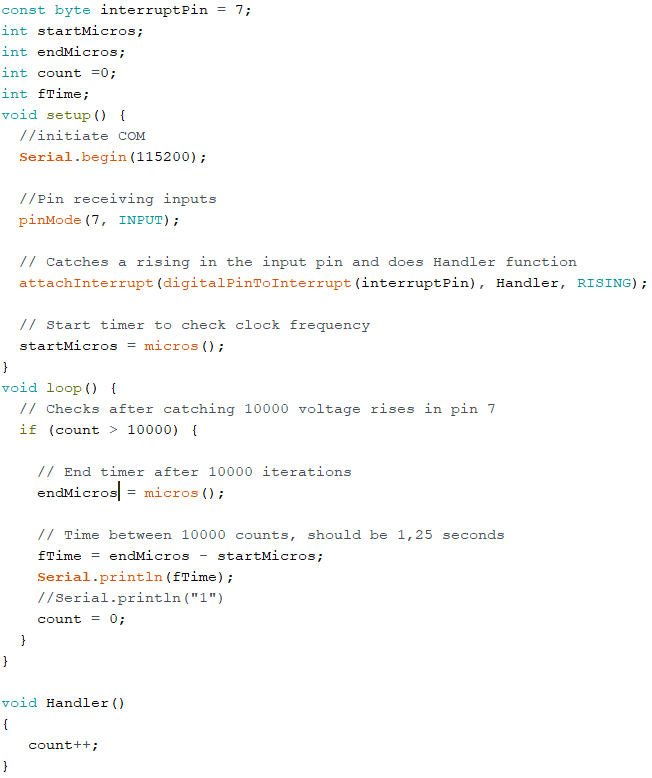
\includegraphics[width=0.85\linewidth]{./sdf/arduino_quantum_rx/figures/arduinoTest.PNG}
	\caption{Arduino test code}
	\label{montage}
\end{figure}

\begin{figure}[H]
	\centering
	\includegraphics[width=1\linewidth]{./sdf/arduino_quantum_rx/figures/Teste2.pdf}
	\caption{Rising edges counts}
	\label{montage}
\end{figure}

\begin{figure}[H]
	\centering
	\includegraphics[width=1\linewidth]{./sdf/arduino_quantum_rx/figures/Teste1.pdf}
	\caption{Time for each 10000 rising edges}
	\label{montage}
\end{figure}
	
	
	\subsubsection{Communication from arduinoReceiver to PC server Netxpto}
	
	To have the set up running we need to open three different programs in the arduino\_real\_time\_receiver paste and run them at the same time: ardRece.ino, serial\_port\_reader\_writer.sln (client side) and netxpto\_qber\_estimation.sln (server side). After the arduino outputs the values of the coincidence block, we need to send the data to a PC, in order to do the calculation of the QBER in real time. To have this implemented in our system, we have the arduino sending the data through the UART one by one to a c++ program in the PC via USB cable. The serial\_port\_reader\_writer.sln program (client side), waits for a connection with the arduino Serial port in order to start receiving the data. Now that the communication between the arduino serial port and the PC is done, the program burns the first 10 seconds of information because the arduino tends to send unnecessary bits when it starts writing in the COM. The program puts the receiving information in a buffer and when it's full all the data is sent to the QBER program . This means we have a TCP/IP connection between the program reading the arduino data and the one that does the QBER calculations. The size of the buffer is 4000 characters. In order to always have the correct values of the QBER we need to have the sequence the arduino is sending synchronized with the sequence from the Alice side. To do this, we have the QBER program running in two modes, the synchronized one, and the unsynchronized. After the program burns the unnecessary data, it is going to check the first few bits in the buffer and compare it with the transmitter sequence. If they are different, the program will discard the first bit that entered the sequence and add a new bit (FIFO). This occurs until we have a match in the sequences, and the program will run normally in the synchronized mode. If, for some reason, the program looses the synchronization, it will do the same process previously explained. In the two modes the program will always  output a file, the midreports, every 8000 bits, with the results of the QBER block calculations. This occurs until we have a match in the sequences, and the program will run normally in the synchronized mode. 
	
	\begin{figure}[H]
		\centering
		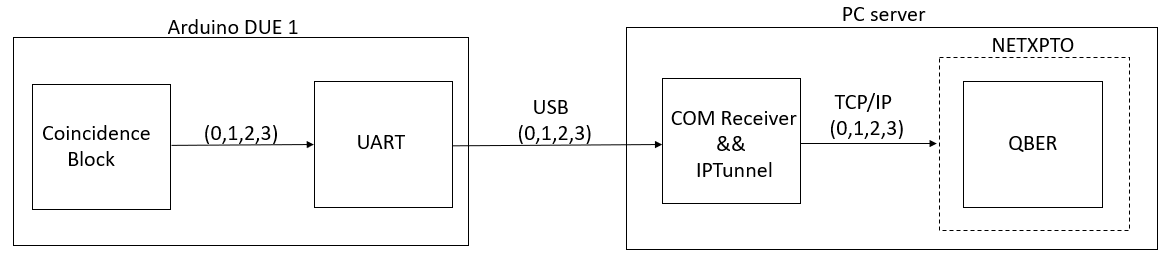
\includegraphics[width=1.1\linewidth]{./sdf/arduino_quantum_rx/figures/PC.png}
		\caption{Block diagram of Arduino to NETXPTO communication.}
		\label{fig:netxpto}
	\end{figure}
	

	As already mention, we need to have the programs running simultaneously. The arduino code simply does the coincidence of the input signals from the detectors, and does a serial print of the four possible results. This print is shown in the COM port of the arduino, and it is possible to send it to a pc through a USB cable. The arduino code is shown below:
	
	\begin{figure}[H]
		\centering
		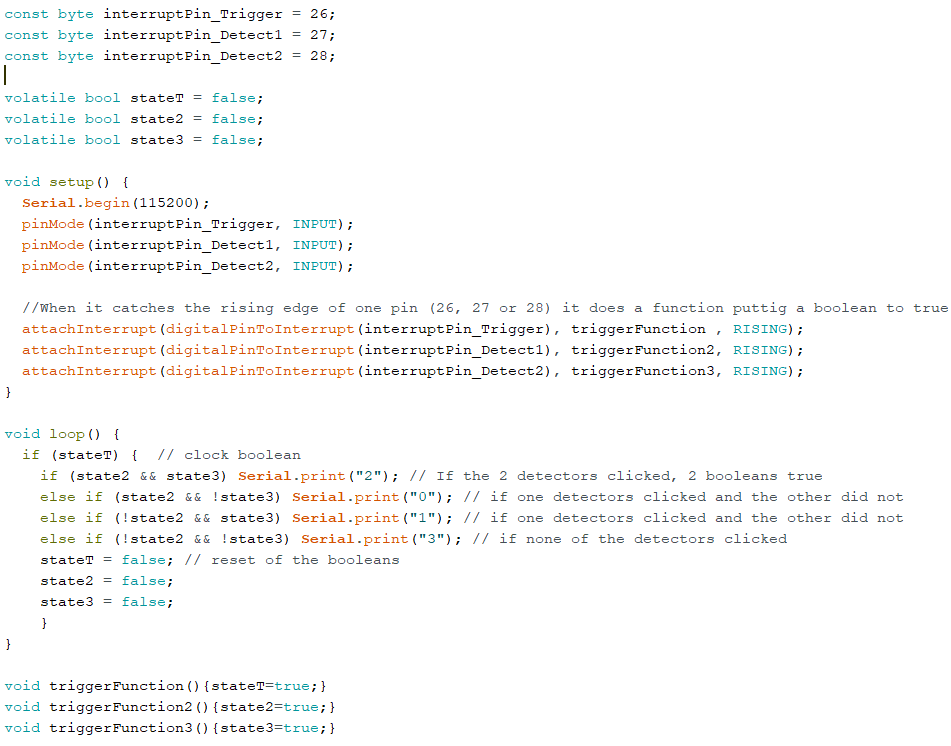
\includegraphics[width=0.85\linewidth]{./sdf/arduino_quantum_rx/figures/arduinoComPC.PNG}
		\caption{Arduino coincidence block and serial communication}
		\label{montage}
		
	\end{figure}

	\clearpage
	
	\subsection{Arduino Implementation - Electronic Polarization Controller }
	Since the communication between the detectors, arduino and NETXPTO is done, now we have to control an EPC, so that Bob can choose in which base he is going to measure the Alice single photons. The new implementation is suggested in the next block diagram, where we added a new arduino, in order to communicate with the NETXPTO, and an external AD5669 DAC. The DAC will output four values of voltages to an EPC, according to the information that comes from the NETXTPO.
	
	\begin{figure}[H] 
		\centering
		\includegraphics[width=1\linewidth]{./sdf/arduino_quantum_rx/figures/Ard.pdf}
		\caption{Block diagram of a arduino implementation.}
		\label{fig:netxpto}
		
	\end{figure}

	\subsubsection{Communication from PC server Netxpto to arduinoTransmitter with DAC}
	In this implementation we also need to control which base Bob is receiving the data. This set up is going to be able to change between four different basis, in which Bob is going to measure the single photons coming from Alice. To have the basis changing, we have to apply four voltages to an EPC. However the arduino only has two internal DACs and needs to receive data from NETXPTO, in order to choose the correct basis. For the first problem, we are using an AD5669 external DAC, that is communicating with the arduino via I2C protocol and can output 8 signals. Also the arduino can't be receiving and sending data through the same serial COM because it will loose synchronism, therefore loosing bits over time. To solve this issue we are using two arduinos: One takes the clock and the output signals and sends them to a PC via USB. The other one also has the clock signal to keep the arduinos synchronized, and it is receiving information from the Netxpto program ,through an USB connection, so that it can choose one set of voltages. However the process of sending data through the PC to the serial COM of the arduino is limited by the PC performance to send information via USB. This means at certain frequencies of the clock, the PC might be doing alot of operations internally affecting the synchronism. The limit of the speed is around 2.5 kHz, which does not represent a problem right now since the system, in a first stage, will be working at 500 Hz. The arduinos need to do all these operations while the detectors are waiting for the next clock pulse. In order to choose the correct basis.
	
	\begin{figure}[H]
		
		\centering
		\includegraphics[width=1\linewidth]{./sdf/arduino_quantum_rx/figures/DAC.png}
		\caption{Block diagram of NETXPTO to EPC communication.}
		\label{fig:netxpto}

	\end{figure}

	Even though we are using two arduinos, we just do some modifications in the arduino program previously presented. Since the implementation uses an external DAC, the arduino needs to communicate with it using a I2C protocol. To do that we need to include the wire library, and use its functions to begin the communication, set the clock speed, write the voltage data to the DAC output and to end the transmission. 
	
	
	\subsection{Open Issues}
	
	\clearpage
	\subsection{Visual Studio 2019 - Installation guide (Current version: 16.2.3)}
	
	\subsubsection{Step 1}
	
	The first thing to do is to download the bootstrapper file of this software through the following link: https://visualstudio.microsoft.com/pt-br/downloads/. As seen below in figure \ref{vstudio} one of three available versions can be choosen.
	
	\begin{figure}[H]
		\centering
		\includegraphics[width=1\linewidth]{./sdf/arduino_quantum_rx/figures/vsDownload.pdf}
		\caption{Download page of Visual Studio IDE software.}
		\label{vstudio}
	\end{figure}
	
	
	\subsubsection{Step 2}
	
	Execute the installer file, which you can use to customize your installation by selecting the feature sets or workloads, individual components, language packs and installation locations, as demonstrated in figure \ref{vstudioWorkloads}.
	
	
	
	\subsubsection{Step 3}
	
	The installation is quite simple and contains few steps for its execution, in case there is any doubt or question you can always get support from https://docs.microsoft.com/en-us/visualstudio/install/install-visual-studio?view=vs-2019.
	
	\begin{figure}[H]
		\centering
		\includegraphics[width=1\linewidth]{./sdf/arduino_quantum_rx/figures/VSworkloads.pdf}
		\caption{Modifying - Visual Studio 2019.}
		\label{vstudioWorkloads}
	\end{figure}
	
	\subsection{Arduino IDE - Installation guide (Current version: 1.8.9) for Windows machines}
	
	\subsubsection{Step 1}
	
	Download the latest version of Arduino desktop IDE installer file from https://www.arduino.cc/en/main/software.
	
	\begin{figure}[H]
		\centering
		\includegraphics[width=0.86\linewidth]{./sdf/arduino_quantum_rx/figures/arduinoDownload.pdf}
		\caption{Download Arduino IDE software.}
		\label{arduinoDownload}
	\end{figure}
	
	
	\subsubsection{Step 2}
	
	When the download finishes, proceed with the installation and allow the driver installation process when you get a warning from the operating system. Follow the help guide present in https://www.arduino.cc/en/Guide/Windows.
	
	\subsubsection{Step 3}
	
	Proceed with the board specific instructions by going to https://www.arduino.cc/en/Guide/HomePage and selecting the respective board from the list provided, for this specific case we are considering the Arduino Due and so you can use the following link: https://www.arduino.cc/en/Guide/ArduinoDue.
	
	\begin{figure}[H]
		\centering
		\includegraphics[width=1\linewidth]{./sdf/arduino_quantum_rx/figures/arduinoBoards.pdf}
		\caption{Select instructions for you specific board, in this case, the Arduino Due.}
		\label{arduinoDownload}
	\end{figure}
	
	\subsection{Visual Micro - Installation and Setup guide}
	Visual Micro is a plugin for Microsoft Visual Studio that helps you creating Arduino compatible cross-platform programs for hundreds of different Arduino compatible micro-controllers. Visual Micro supports projects that contain one or more .ino code files and standard c++ cource code files, just like the Arduino IDE.
	
	
	\subsubsection{Step 1}
	Download Visual Micro from here https://www.visualmicro.com/page/Arduino-Visual-Studio-Downloads.aspx or it can also be installed and uninstalled from inside the IDE, by opening Visual Studio and clicking "Extensions>Manage Extensions>Online>Arduino IDE for Visual Studio".
	
	\subsubsection{Step 2}
	If Visual Studio/Atmel Studio is running, then close it.
	
	\subsubsection{Step 3}
	Install Visual Micro by doubleclicking on the "vsix" icon of the downloaded file or in the case you are installing it from within the Visual Studio IDE it will start automatically.
	
	\subsubsection{Step 4}
	
	The first time, after you have installed Arduino for Visual Micro, the Configuration Manager will pop up where you can configure your system. Visual Micro must know the version and installation path of the Arduino IDE software that you have installed in your computer.
	
	\begin{figure}[H]
		\centering
		\includegraphics[width=1\linewidth]{./sdf/arduino_quantum_rx/figures/configureIDE.pdf}
		\caption{Configure IDE locations.}
		\label{configureIDE}
	\end{figure}
	
	\subsubsection{Step 4}
	If you work with different boards that required different IDEs, or if you have multiple versions of the Arduino IDE installed, then repeat the steps above for each IDE. It is possible to switch between configurations with the toolbar presented below in figure \ref{}.
	
	\begin{figure}[H]
		\centering
		\includegraphics[width=0.7\linewidth]{./sdf/arduino_quantum_rx/figures/multipleIDEversions.pdf}
		\caption{Support for Multiple Versions of the Arduino Softwares.}
		\label{multipleIDEversions}
	\end{figure}
	
	
	\subsubsection{Step 5}
	
	In order to select the board model use the Visual Micro "Micro Boards" toolbar for that purpose, presented below. If the Visual Micro toolbar is missing, then you can show it by right clicking on an empty space in the toolbar area and checking "Micro Boards".
	
	
	\begin{figure}[H]
		\centering
		\includegraphics[width=0.7\linewidth]{./sdf/arduino_quantum_rx/figures/boardSelect.pdf}
		\caption{Selecting the Board Model.}
		\label{boardSelect}
	\end{figure}
	
	\subsubsection{Step 6}
	
	Connect your Arduino board to your PC using a USB cable. You must also tell your IDE which serial port to use and for that purpose use the Visual Micro Serial Communications toolbar shown below in figure \ref{selectSerial}. If the Visual Micro Serial Communications toolbar is missing, then you can show it by right clicking in the toolbar area and checking "Micro Serial Communications".
	
	\begin{figure}[H]
		\centering
		\includegraphics[width=0.7\linewidth]{./sdf/arduino_quantum_rx/figures/selectSerial.pdf}
		\caption{Setting up your Serial Port.}
		\label{selectSerial}
	\end{figure}
	
	\subsubsection{Step 7}
	At the end of these steps, you will be ready to write, compile, debug, and upload your Arduino sketches. In case of doubts consult the following link: https://www.visualmicro.com/page/User-Guide.aspx?doc=index.
	
	% bibliographic references for the section ----------------------------
	\clearpage
	\printbibliography[heading=subbibliography]
\end{refsection}
\addcontentsline{toc}{subsection}{Bibliography}
\cleardoublepage
% ---------------------------------------------------------------------
